\documentclass[tikz,border=5]{standalone}
\begin{document}
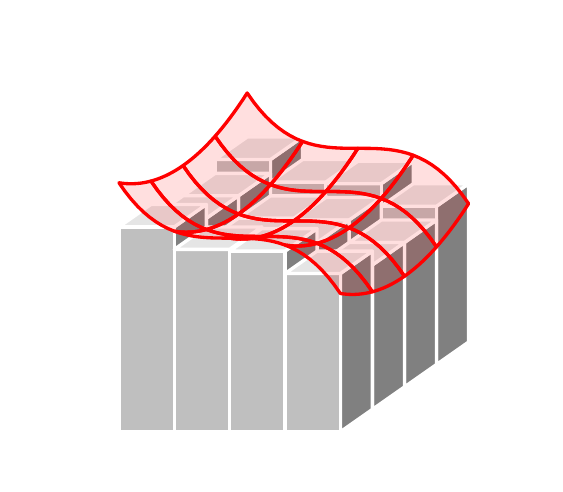
\begin{tikzpicture}[
  x=(215:2em/sqrt 2), y=(0:2em), z=(90:2em),
  declare function={f(\x,\y)=((\x-3)^2+(-\y+3)^3)/8+3;}, 
  very thick, line join=round]
\draw [-stealth, white] (0,0,0) -- (5,0,0) node [below left] {$x$};
\draw [-stealth, white] (0,0,0) -- (0,5,0) node [below right] {$y$};
\draw [-stealth, white] (0,0,0) -- (0,0,5) node [right] {$z$};
\foreach \x in {1,...,4}
  \foreach \y [evaluate={\j=\x+.5; \i=\y+.5; \k=f(\j,\i);}] in {1,...,4}{
    \path [fill=black!50, draw=white] (\x, \y+1, 0) -- (\x+1, \y+1, 0) -- 
      (\x+1, \y+1, \k) -- (\x, \y+1, \k) -- cycle;
    \path [fill=black!25, draw=white] (\x+1, \y, 0) -- (\x+1, \y+1, 0) -- 
      (\x+1, \y+1, \k) -- (\x+1, \y, \k) -- cycle;
    \path [fill=black!10, draw=white] (\x, \y, \k)  -- (\x+1, \y, \k) -- 
      (\x+1, \y+1, \k) -- (\x, \y+1, \k) -- cycle;
  }
 \foreach \x in {1,...,4}
   \foreach \y in {1,...,4}{
 \draw [red, fill=red, fill opacity=0.125, 
    domain=0:1, samples=10, variable=\t] 
    plot (\x+\t, \y, {f(\x+\t,\y)}) -- 
    plot (\x+1, \y+\t, {f(\x+1,\y+\t)}) -- 
    plot (\x+1-\t, \y+1, {f(\x+1-\t,\y+1)}) --
    plot (\x, \y+1-\t, {f(\x,\y+1-\t)}) -- cycle;
  }
\end{tikzpicture}
\end{document}